\chapter{Evaluation}
\label{chp:chapter_4}
The evaluation of our system is split up in a \textit{static} and a \textit{dynamic} part. The static evaluation quantifies the connection setup performance for each optimization stage. The static behavior will be benchmarked on \textit{number of packets during connection setup}, \textit{connection setup time}, and \textit{time until first useful packet}. The dynamic evaluation is about quantifying the performance of FRAPPUCcInO, which will be based on \textit{average throughput}, and \textit{responsiveness}.

This separation is made because the static performance improvement will be applicable to both intermittently-powered and conventionally-powered devices. Reducing connection setup time and power consumption on their own are attractive propositions since it improves responsiveness and battery life. The FRAPPUCcInO algorithm is not the only possible application of \textit{Fast Reconnect}. For example, Fast Reconnect could also be leveraged to quickly build a connection when ambient energy is insufficient for even the maximum connection interval, allowing a pseudo-connected state. 

\section{Experimental Setup}
\label{sec:evaluation_setup}
The demo application described in Section \ref{sec:demo_application} was also used for all experiments. The central is an nRF52840DK development board, and the peripheral is the modified FreeBie platform. The nRF52840-Dongle was used as a sniffer for Wireshark. During the static testing, the Nordic Power Profiler Kit II (PPK-II) was used to power FreeBie and measure its power consumption. During the dynamic testing, the PPK-II was replaced with a 46.5$\mu\text{W}$ solar cell from Panasonic \cite{panasonic_solar}, and a Saleae Logic Pro 8 was used to capture digital and analog traces \cite{saleae_logic_pro_8}. Finally, an Ikea TRÅDFRI smartlight was calibrated and controlled through \texttt{python} to simulate changing energy harvesting conditions. 

The \texttt{CMakeLists} file has been retrofitted to enable easy switching between optimization stages during testing. Set the \texttt{CMake} variables according to Table \ref{tbl:stage_defs} to enable a specific stage.
\begin{table}
    \begin{center}
    \begin{tabular}{|l|l|l|l|l|}
        \hline
                                & \multicolumn{4}{c|}{\textbf{Stage}}   \\
        \textbf{Variable}    & \textbf{1} & \textbf{2} & \textbf{3} & \textbf{4} \\
        \hline
        CACHE\_SERVICE\_DISCOVERY &   & 1 & 1 & 1 \\
        \hline
        SKIP\_RECONF             &   &   & 1 & 1 \\
        \hline
        CACHE\_LL\_FEAT\_EXCH      &   &   &   & 1 \\
        \hline
        CACHE\_LL\_DL\_EXCH        &   &   &   & 1 \\
        \hline
    \end{tabular}
    \end{center}
    \caption{\texttt{CMake} variables to set for a given optimization stage. Set the variable to 1 if the cell contains a 1, otherwise do not set the variable.}
    \label{tbl:stage_defs}
\end{table}

\section{Results}
\label{sec:evaluation_results}

\subsection{Static}
\label{sec:static_evaluation}


% Number of Packets Plot
\pgfplotsset{
    compat=1.9,
    compat/bar nodes=1.8,
}
\pgfplotstableread{
    Label Discovery Configuration Link-layer emptypdu Application
    0     58        8             9          6        2
    1     58        8             9          7        2
    2     6         8             9          10       5
    3     0         0             9          3        5
    4     0         0             1          0        0
}\connsetupdata
\begin{figure}
    \begin{center}
    \begin{tikzpicture}
        \begin{axis}[
            ybar stacked,
            ymin=0,
            ymax=100,
            xtick=data,
            legend style={
                cells={anchor=west},
                legend pos=north east,
            },
            reverse legend=true,
            xticklabels from table={\connsetupdata}{Label},
            xticklabel style={text width=2cm,align=center},
        ]
            \addplot [fill=green!80]
                table [y=Discovery, meta=Label, x expr=\coordindex]
                    {\connsetupdata};
                        \addlegendentry{Discovery}
            \addplot [fill=blue!60]
                table [y=Configuration, meta=Label, x expr=\coordindex]
                    {\connsetupdata};
                        \addlegendentry{Configuration}
            \addplot [fill=red!60]
                table [y=Link-layer, meta=Label, x expr=\coordindex]
                    {\connsetupdata};
                        \addlegendentry{Link Layer}
            \addplot [fill=gray!60]
                table [y=emptypdu, meta=Label, x expr=\coordindex]
                    {\connsetupdata};
                        \addlegendentry{Empty PDU}
            \addplot [fill=purple!60,nodes near coords,point meta=y]
                table [y=Application, meta=Label, x expr=\coordindex]
                    {\connsetupdata};
                        \addlegendentry{Application}
        \end{axis}
    \end{tikzpicture}
\end{center}
\caption{Division of Packets for Levels of Optimization}
\label{fig:division_packets}
\end{figure}


% Setup Time Plot
\pgfplotsset{
    compat=1.9,
    compat/bar nodes=1.8,
}
\pgfplotstableread{
    Label SetupTime 
    0     1.862        
    1     134.762     
    2     37.591   
    3     15.997    
    4     0.001    
}\setuptimedata
\begin{figure}
    \begin{center}
\begin{tikzpicture}
    \begin{axis}[
        ybar,
        ymin=0,
        ymax=150,
        xtick=data,
        xticklabels from table={\setuptimedata}{Label},
        xticklabel style={text width=2cm,align=center},
    ]
        \addplot [fill=green!60,nodes near coords,point meta=y]
            table [y=SetupTime, meta=Label, x expr=\coordindex]
                {\setuptimedata};
    \end{axis}
\end{tikzpicture}
\end{center}
\caption{Connection Setup Time}
\end{figure}

% Time To Useful Packet Plot
\pgfplotsset{
    compat=1.9,
    compat/bar nodes=1.8,
}
\pgfplotstableread{
    Label Time 
    0     5.021
    1     136.762  
    2     25.994
    3     4.800
    4     6.445
}\timetousefuldata
\begin{figure}
    \begin{center}
        \begin{tikzpicture}
            \begin{axis}[
                ybar,
                ymin=0,
                ymax=150,
                xtick=data,
                xticklabels from table={\timetousefuldata}{Label},
                xticklabel style={text width=2cm,align=center},
            ]
                \addplot [fill=blue!60,nodes near coords,point meta=y]
                    table [y=Time, meta=Label, x expr=\coordindex]
                        {\timetousefuldata};
            \end{axis}
        \end{tikzpicture}
    \end{center}
    \caption{Time Until Useful Packet}
\end{figure}


% Connection Adaption Time vs. current CI
\begin{figure}
    \begin{center}
    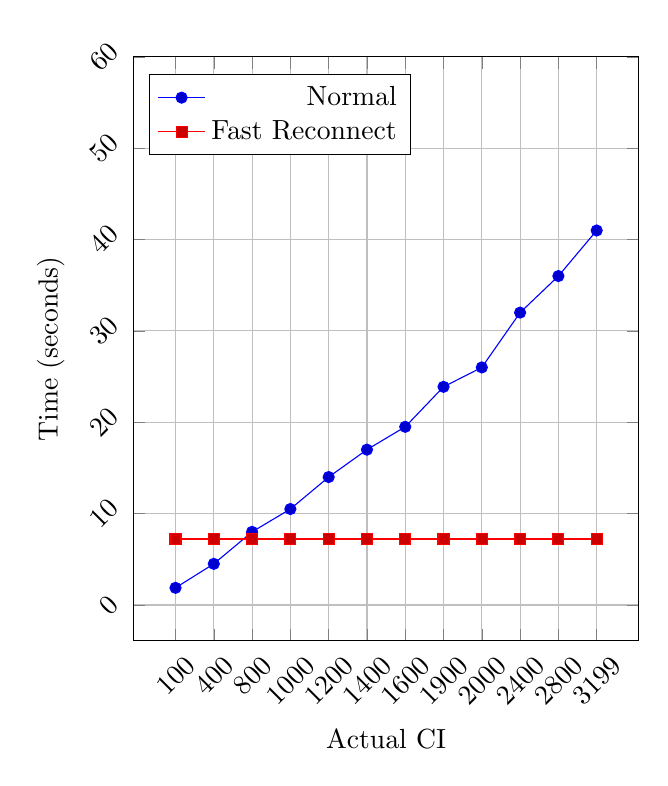
\begin{tikzpicture}
    \begin{axis}[
    ymax = 60,
    symbolic x coords={100, 400, 800, 1000, 1200, 1400, 1600, 1900, 2000, 2400, 2800, 3199},
    xtick=data,
    height=9cm,
    width=8cm,
    grid=major,
    xlabel={Actual CI},
    ylabel={Time (seconds)},
    legend style={
    cells={anchor=east},
    legend pos=north west,
    tick label style={rotate=45} % <-- this is added
    }
    ]
    
    \addplot coordinates {
        (100,1.875)
        (400,4.5)
        (800,8)
        (1000,10.5)
        (1200,14)
        (1400,17)
        (1600,19.5)
        (1900,23.876)
        (2000,26)
        (2400,32)
        (2800,36)
        (3199,40.989)
    };
    \addplot coordinates {
        (100,7.22)
        (400,7.22)
        (800,7.22)
        (1000,7.22)
        (1200,7.22)
        (1400,7.22)
        (1600,7.22)
        (1900,7.22)
        (2000,7.22)
        (2400,7.22)
        (2800,7.22)
        (3199,7.22)
    };
    
    
    \legend{Normal, Fast Reconnect}
\end{axis}
\end{tikzpicture}
\end{center}
        \caption{Connection Adaption Time}
\end{figure}

\subsection{Dynamic}
\label{sec:static_evaluation}